\documentclass{article}
\usepackage[utf8]{inputenc}
\usepackage{graphicx}

\title{CW13}
\author{Jacob Anabi and Gage Kizzar }
\date{December 2018}

\begin{document}

\maketitle

\section{Abstract}
In this paper, we attempt to solve, plot, and interpret a two coupled set of ODES, also known as the 'Duffing oscillator':

$$\dot{x}(t) = y(t)$$
$$m\dot{y}(t) = -\nu y(t) + x(t) - x^3(t) + F\cos(\omega t)$$

We will solve these equations numerically, for $m=1$, $\nu = 0.25$, and $\omega = 1$, using a time-step size of $\Delta t = 0.001$ with the 4th-order Runge-Kutta integration method. We will be adjusting $x_0$, $y_0$, $F$, and the domain $t$.

\section{Introduction}
Let's consider a ball of mass $m$ with horizontal coordinate $x$ rolling in a double-well potential $V(x) = x^4/4 - x^2/2$. We will jiggle the ball at the bottom of the well. Thus, the ball, according to Newton's Second Law of Motion, must satisfy the following equation:

$$m\ddot{x} = f_{\text{hat}}(x) + f_{\text{drag}}(\dot{x}) + f_{\text{drive}}(t) = x - x^3 - \nu \dot{x} + F\cos(\omega t)$$

We can split this into two coupled first-order ODEs:

$$\dot{x}(t) = y(t)$$
$$m\dot{y}(t) = -\nu y(t) + x(t) - x^3(t) + F\cos(\omega t)$$

\section{Plots and Interpretation}

$F=0.18$, $x(0)=-0.9$, and $y(0)=0$

\begin{figure}[h!]
\centering
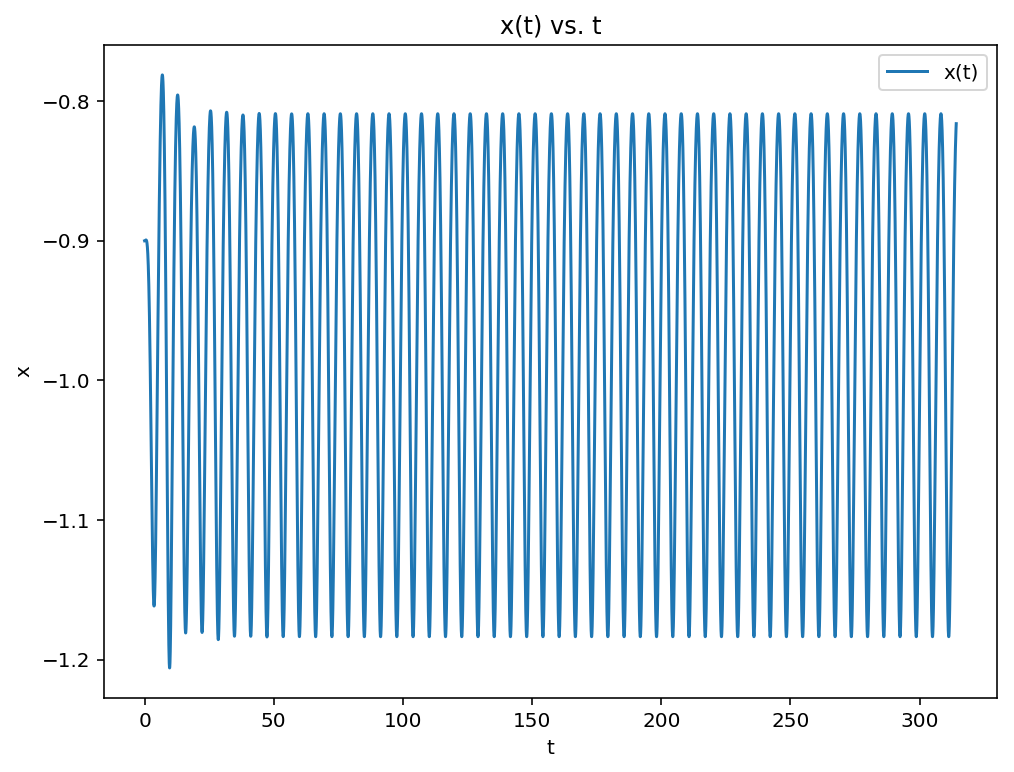
\includegraphics[scale=0.4]{x(t)1.png}
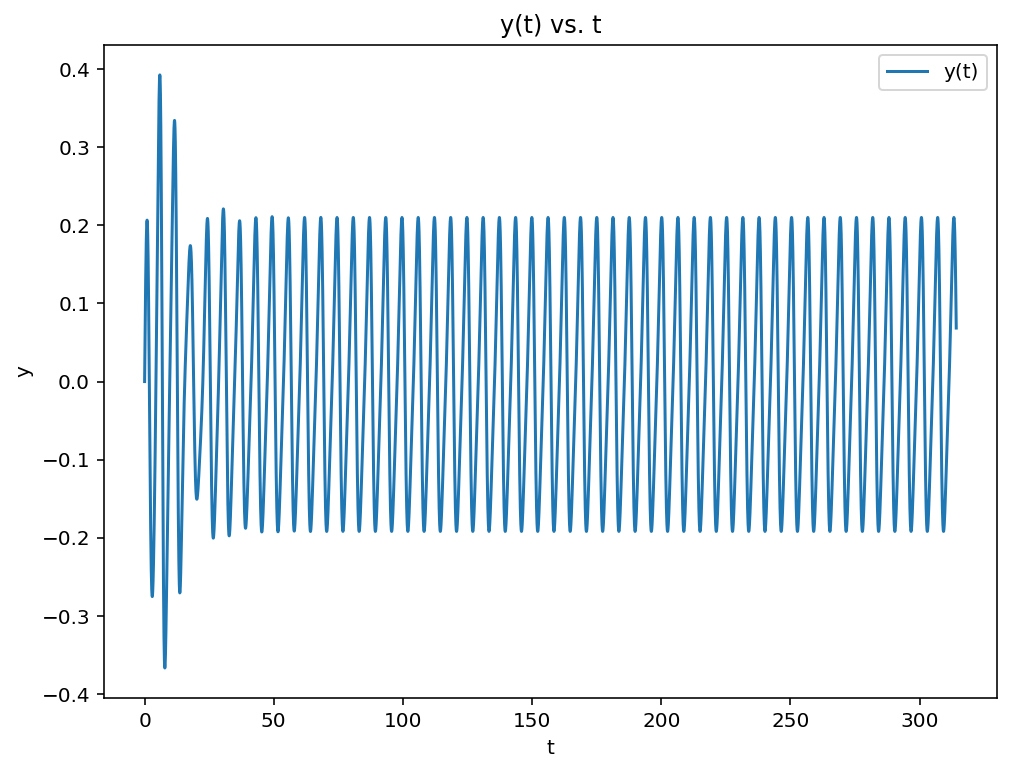
\includegraphics[scale=0.4]{y(t)1.png}
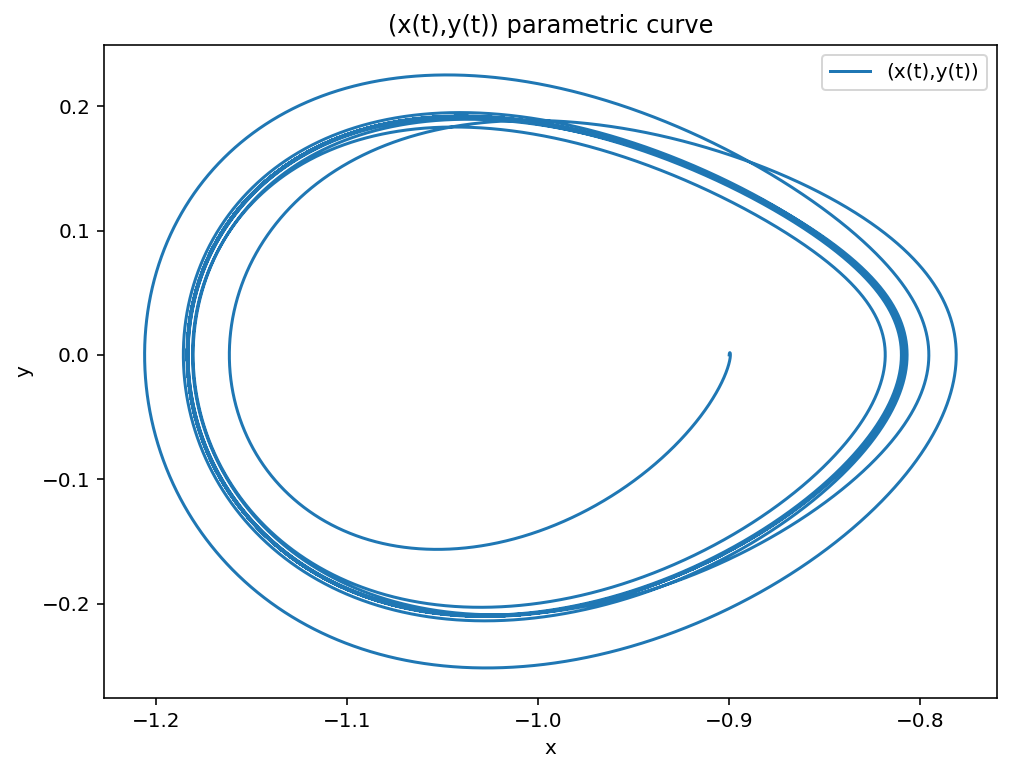
\includegraphics[scale=0.4]{parametriccurve1.png}
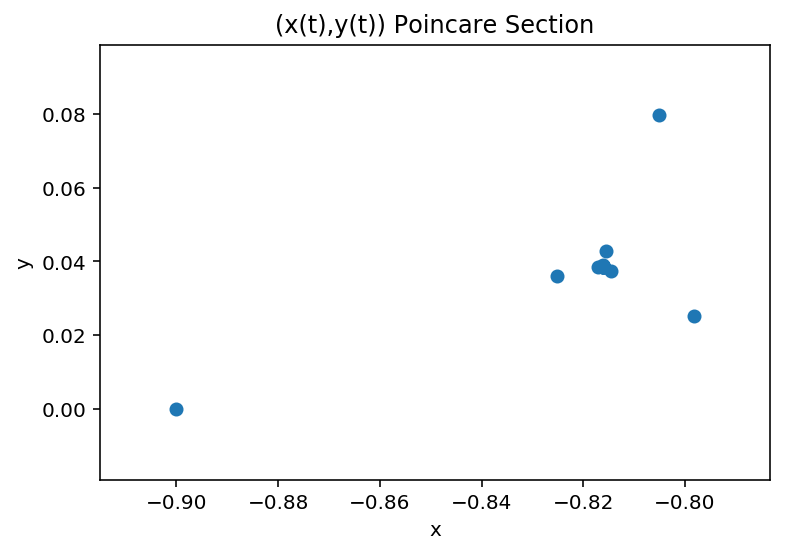
\includegraphics[scale=0.4]{poincare1.png}
\end{figure}

By examining our $t\,\, vs.\,\, x(t)$ and $t\,\, vs.\,\, y(t)$ graph, we can see some sort of oscillation, which is expected from our system. The system appears periodic. The Poincare section shows the system clustering at a single point.

$F = 0.18$, $x(0) = 0.9$, and $y(0) = 0$

\begin{figure}[h!]
\centering
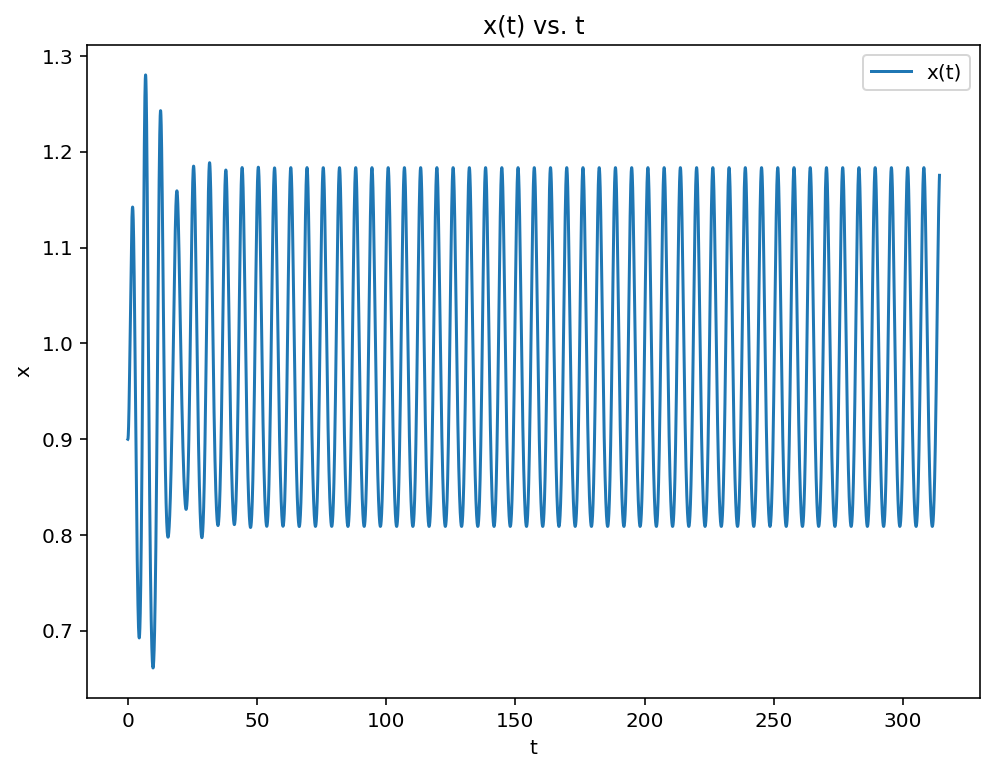
\includegraphics[scale=0.4]{x(t)2.png}
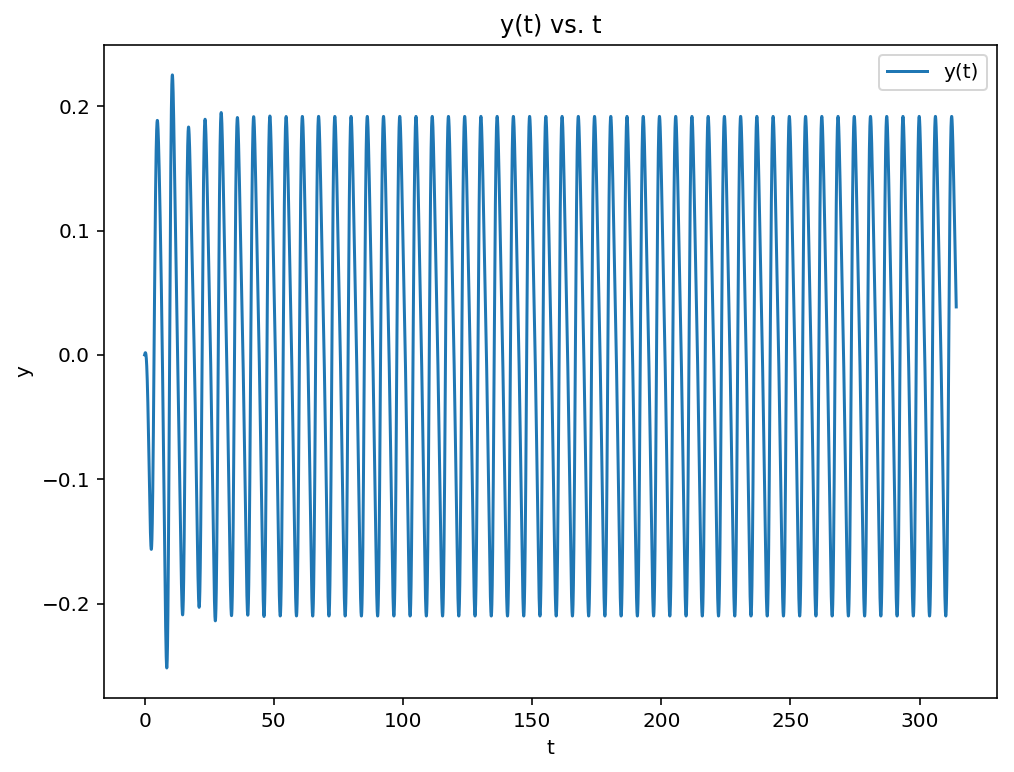
\includegraphics[scale=0.4]{y(t)2.png}
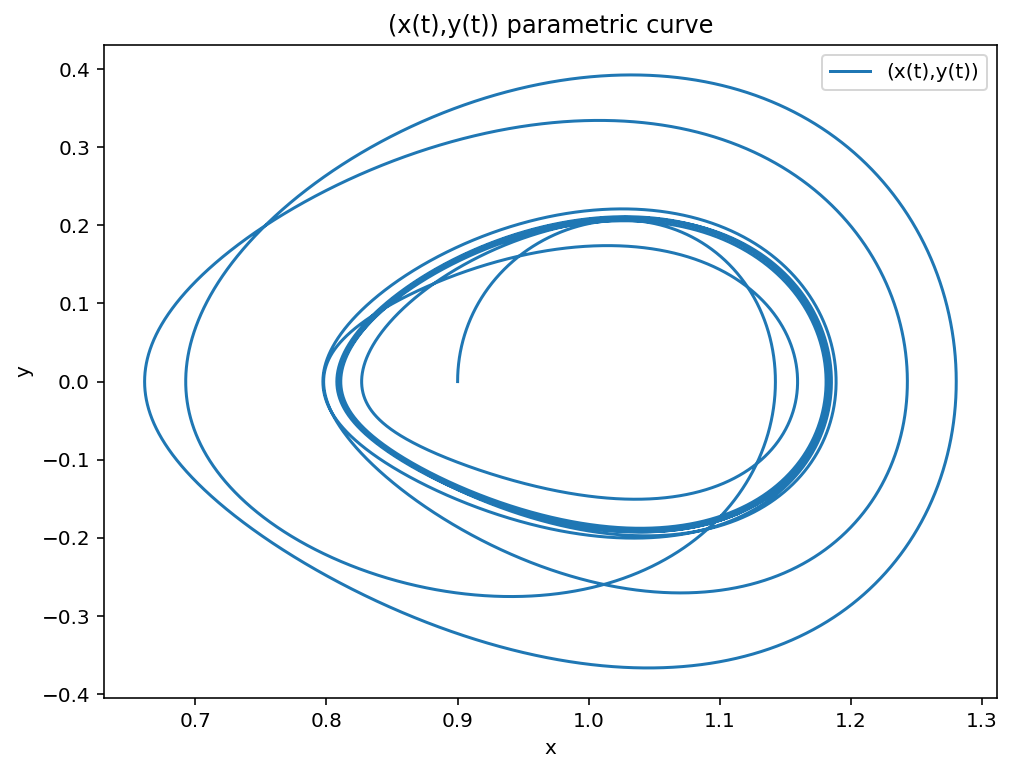
\includegraphics[scale=0.4]{parametriccurve2.png}
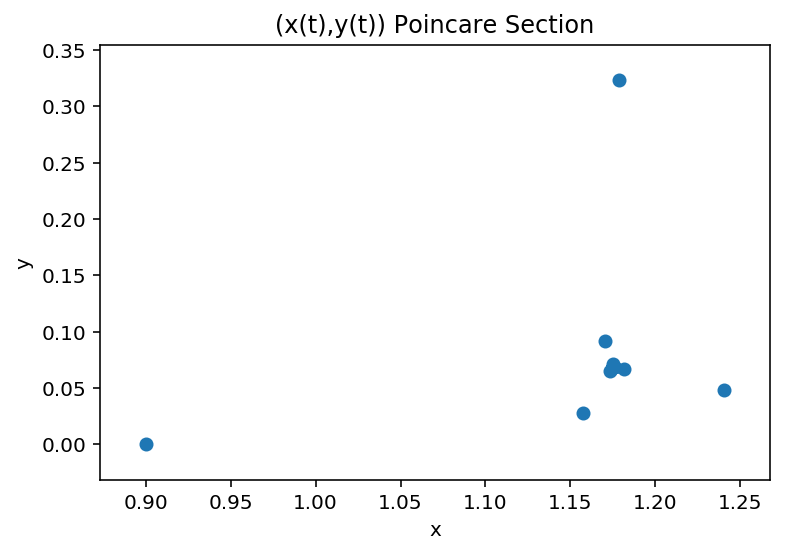
\includegraphics[scale=0.4]{poincare2.png}
\end{figure}

Changing our initial $x-value$ has led to our system clustering at a different point in the well.

$F = 0.25$, $x(0) = 0.2$, and $y(0) = 0.1$

\begin{figure}[h!]
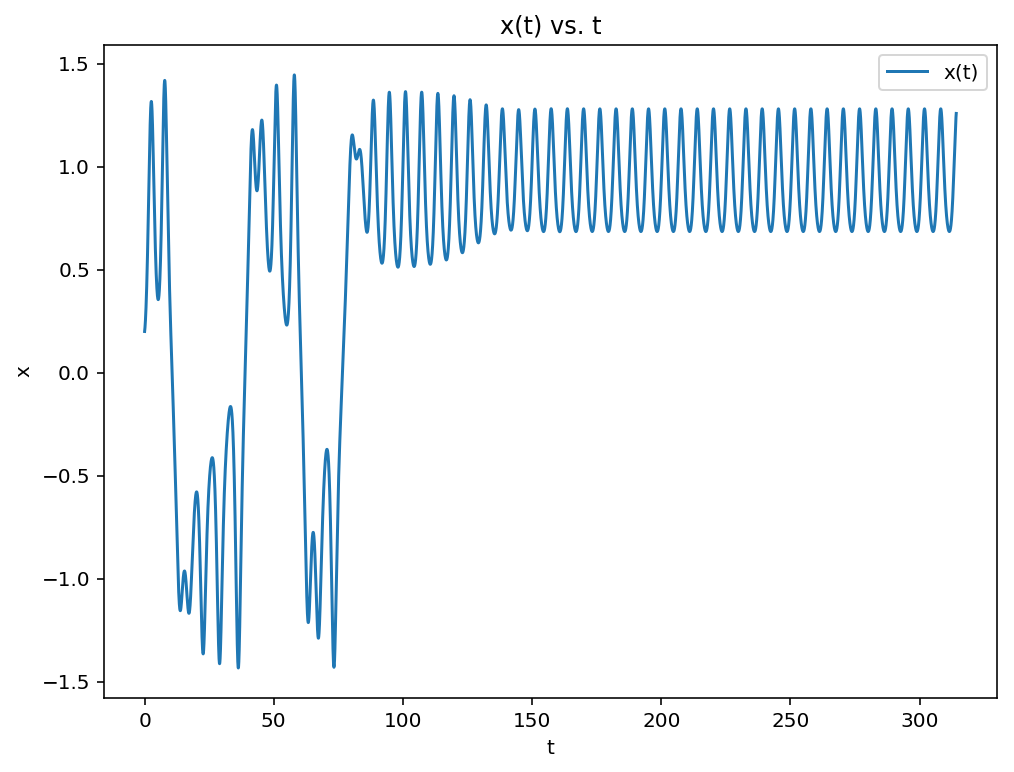
\includegraphics[scale=0.4]{x(t)3.png}
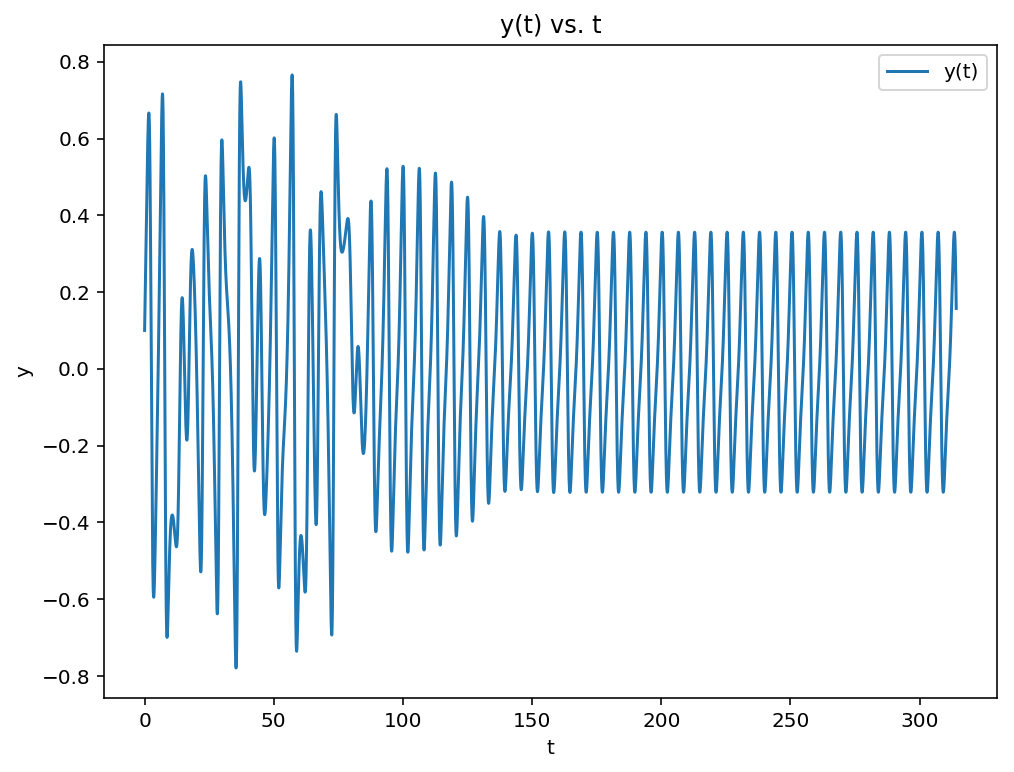
\includegraphics[scale=0.4]{y(t)3.png}
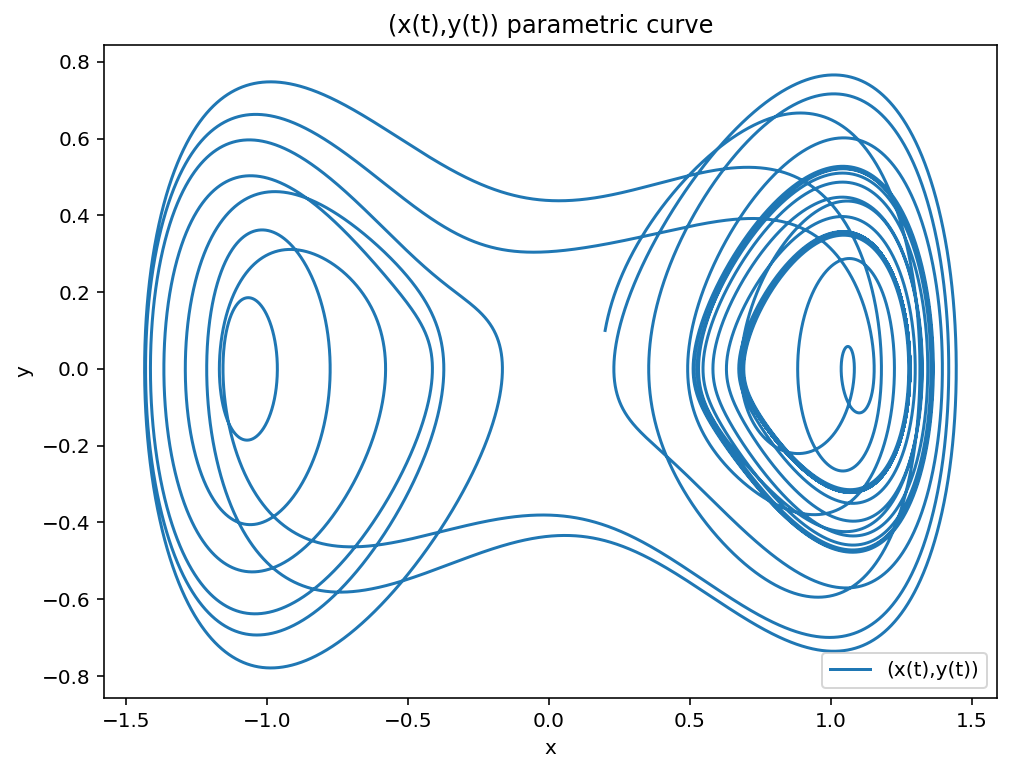
\includegraphics[scale=0.4]{parametriccurve3.png}
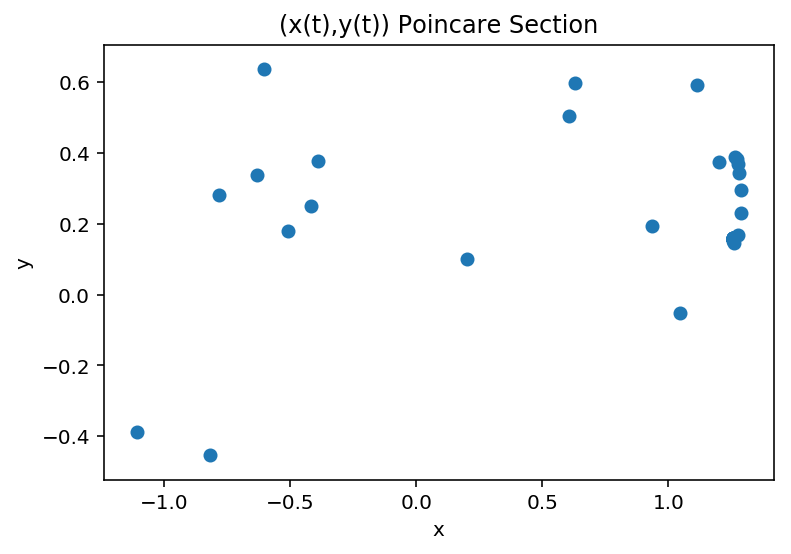
\includegraphics[scale=0.4]{poincare3.png}
\end{figure}

Changing our $F-value$ and initial $x-value$ and $y-value$ seems to create a slightly chaotic system; it is getting harder to examine a pattern in Poincare section compared to our previous plots. Additionaly, the object seems to attract more to the right side of the well. We will test this by tweaking the initial condition very slightly.

$F = 0.25$, $x(0) = 0.201$, and $y(0) = 0.1$

\begin{figure}[h!]
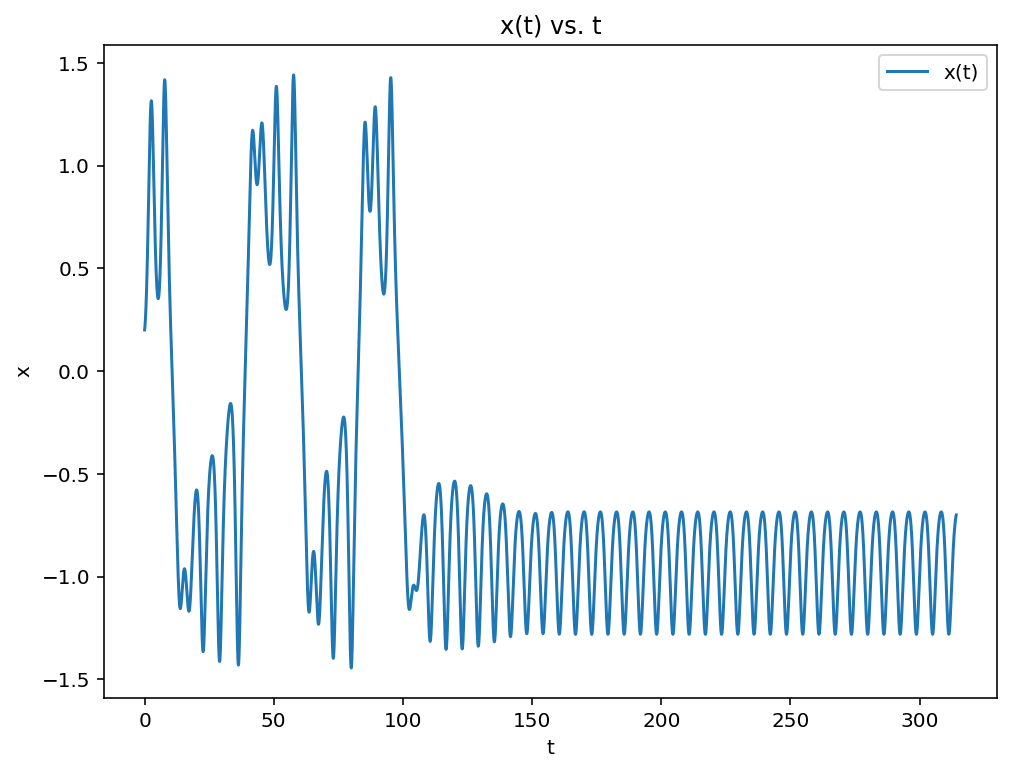
\includegraphics[scale=0.4]{x(t)4.png}
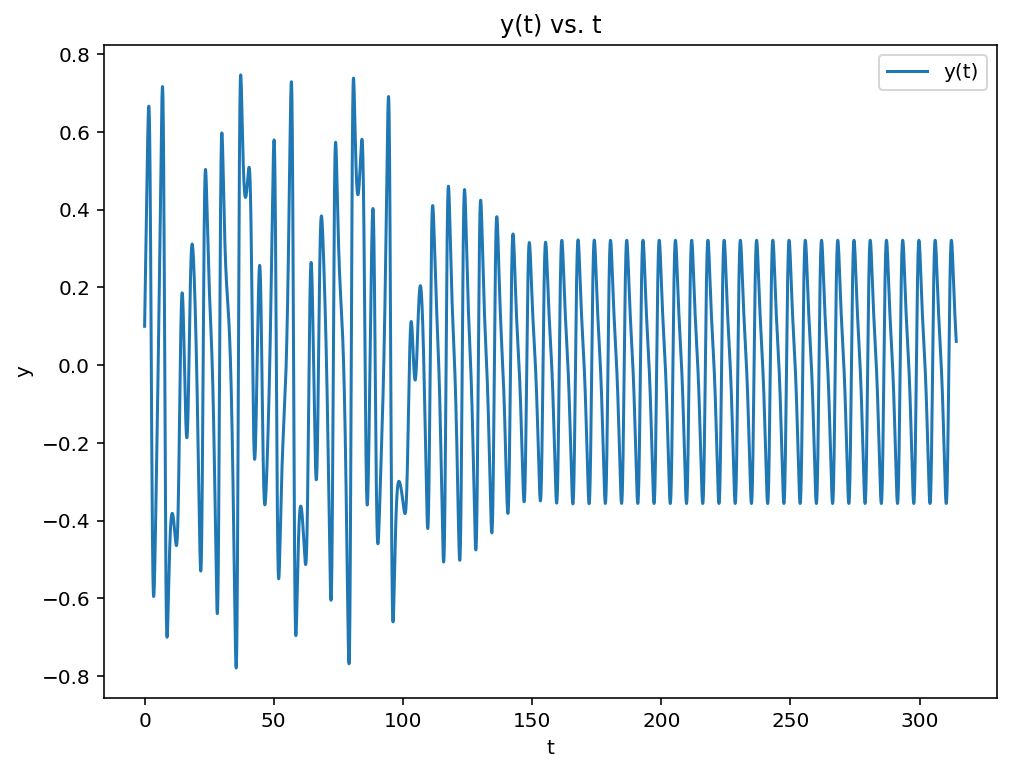
\includegraphics[scale=0.4]{y(t)4.png}
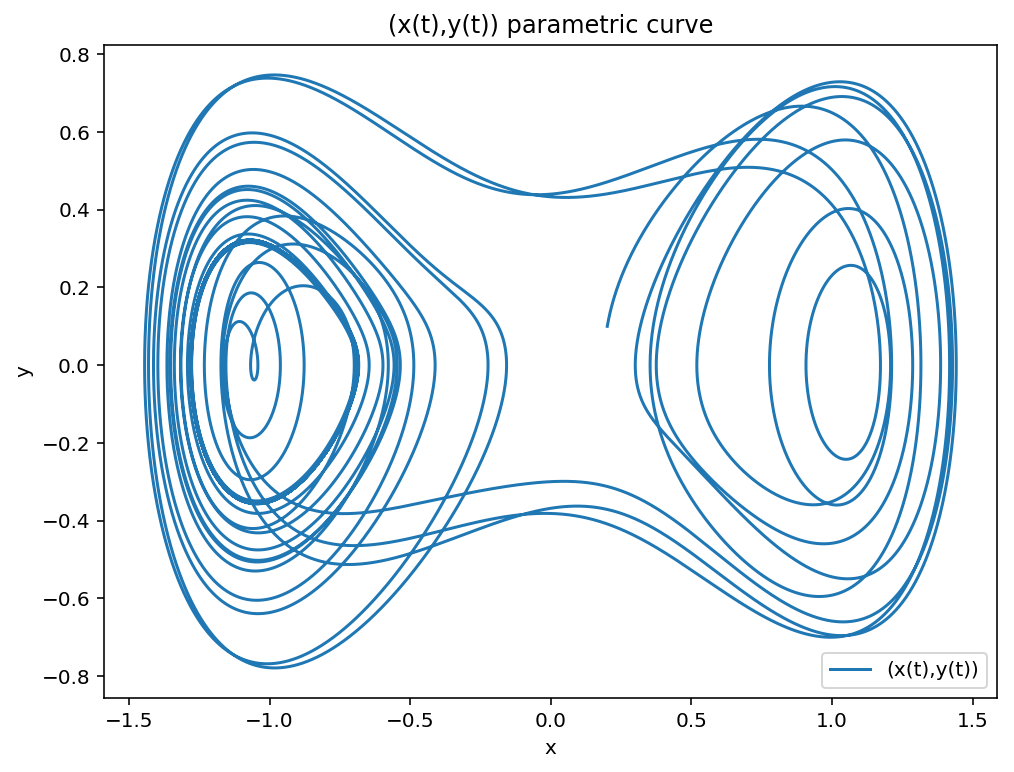
\includegraphics[scale=0.4]{parametriccurve4.png}
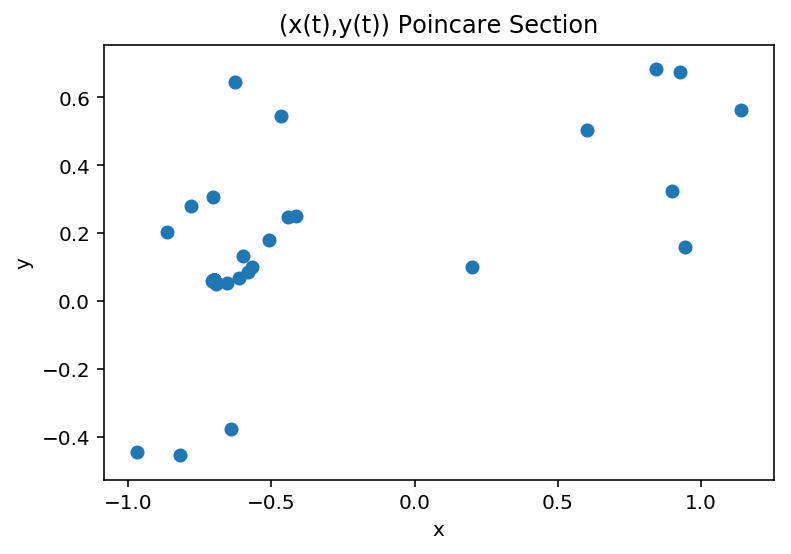
\includegraphics[scale=0.4]{poincare4.png}
\end{figure}

As we can see, changing our initial condition resulted in a wildly different outcome. The object nows seems more attracted to the left side of the will. This seems to be an indication of a chaotic system.

$F = 0.4$, $x(0) = 0$, and $y(0) = 0$

\begin{figure}[h!]
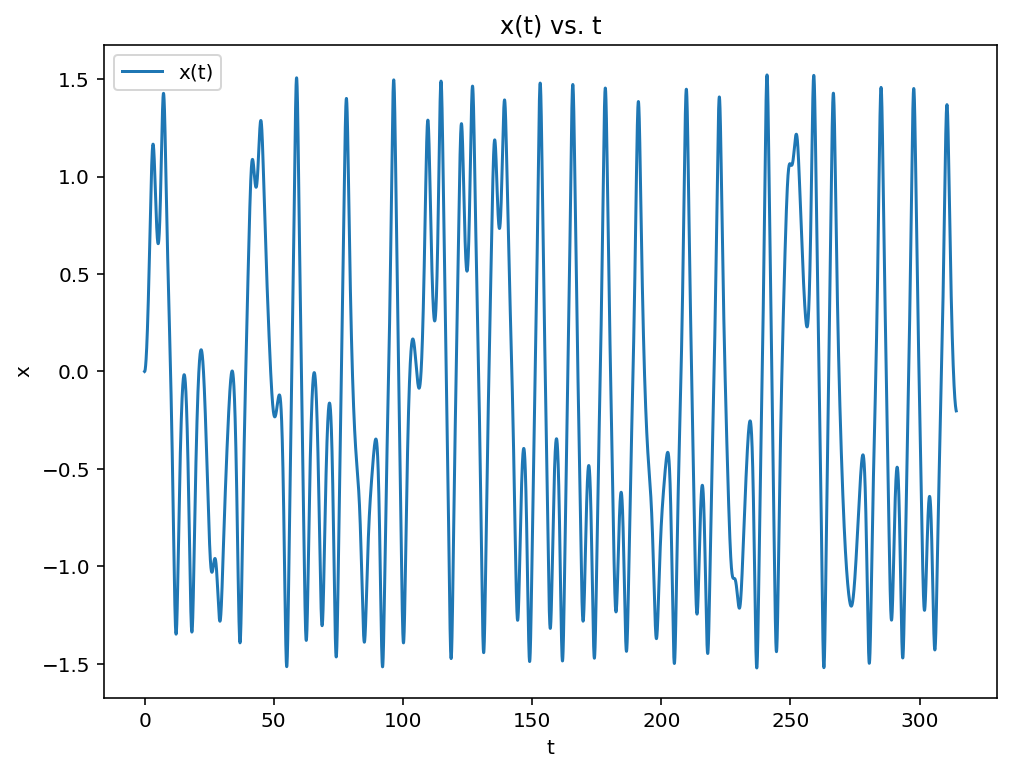
\includegraphics[scale=0.4]{x(t)5.png}
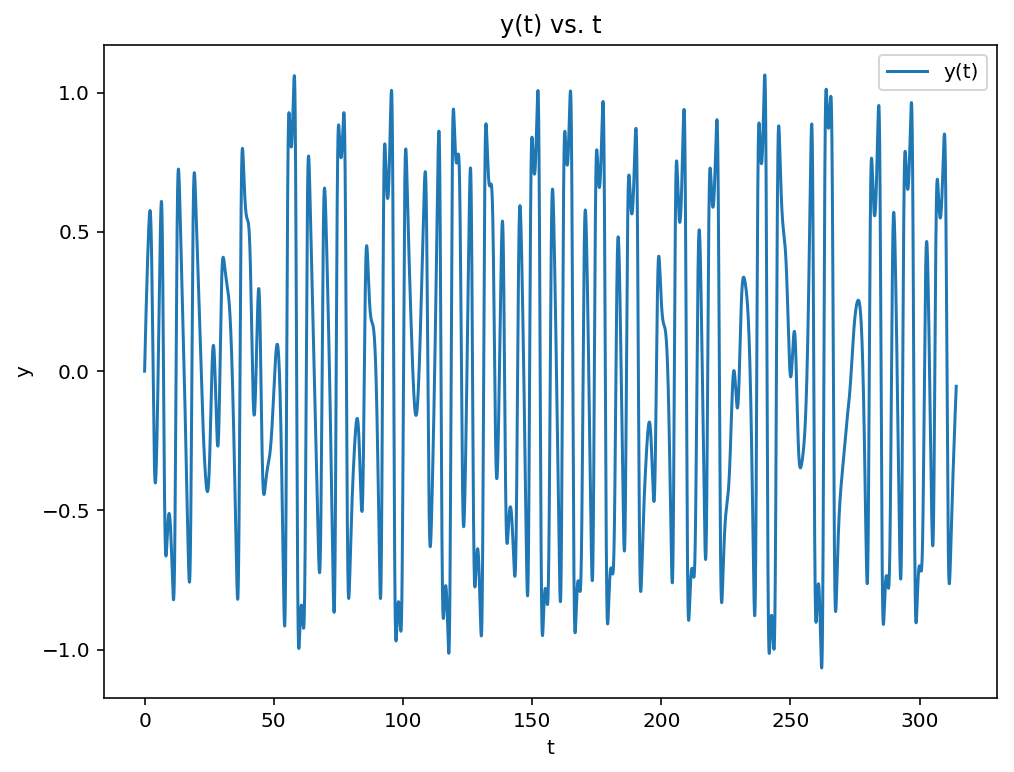
\includegraphics[scale=0.4]{y(t)5.png}
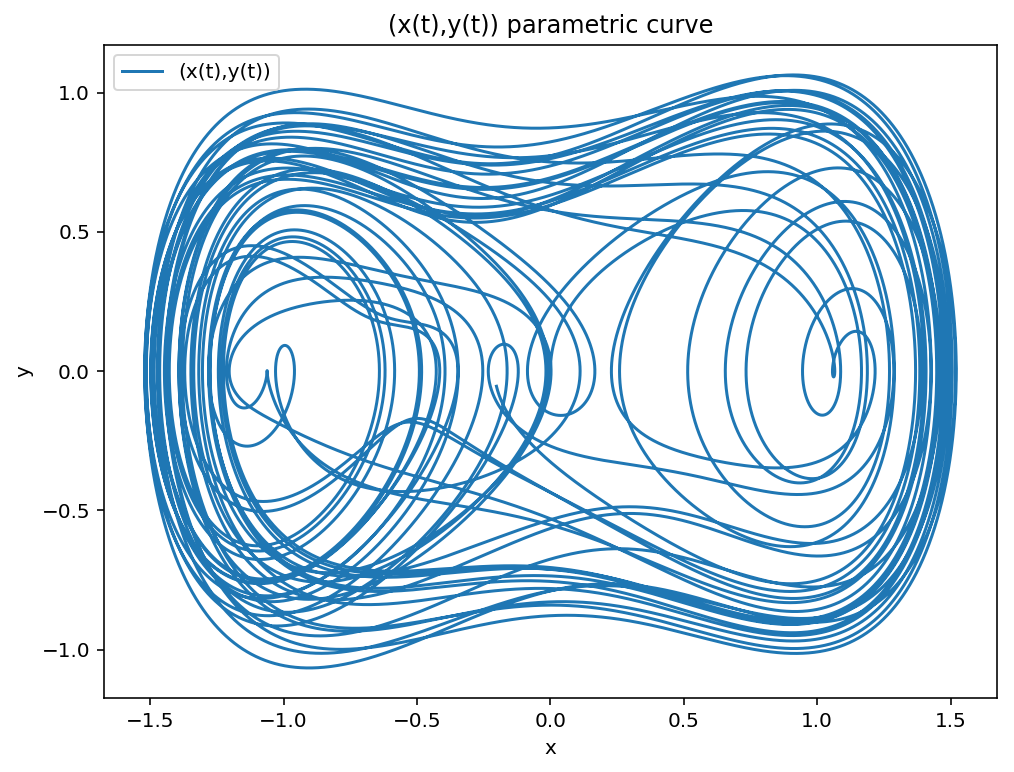
\includegraphics[scale=0.4]{parametriccurve5.png}
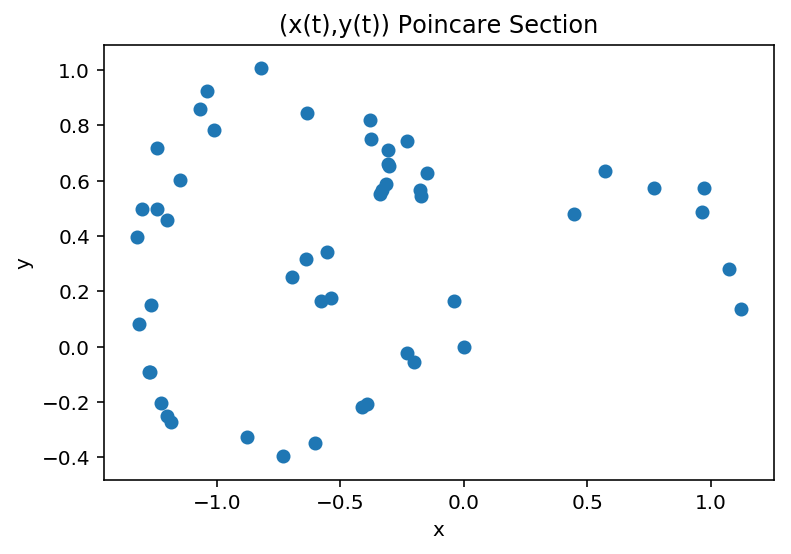
\includegraphics[scale=0.4]{poincare5.png}
\end{figure}

We can now clearly see chaotic behavior. We cannot discern a clear pattern in our Poincare section. Let's try tweaking our initial conditions slightly.

$F = 0.4$, $x(0) = 0.001$, and $y(0) = 0$

\begin{figure}[h!]
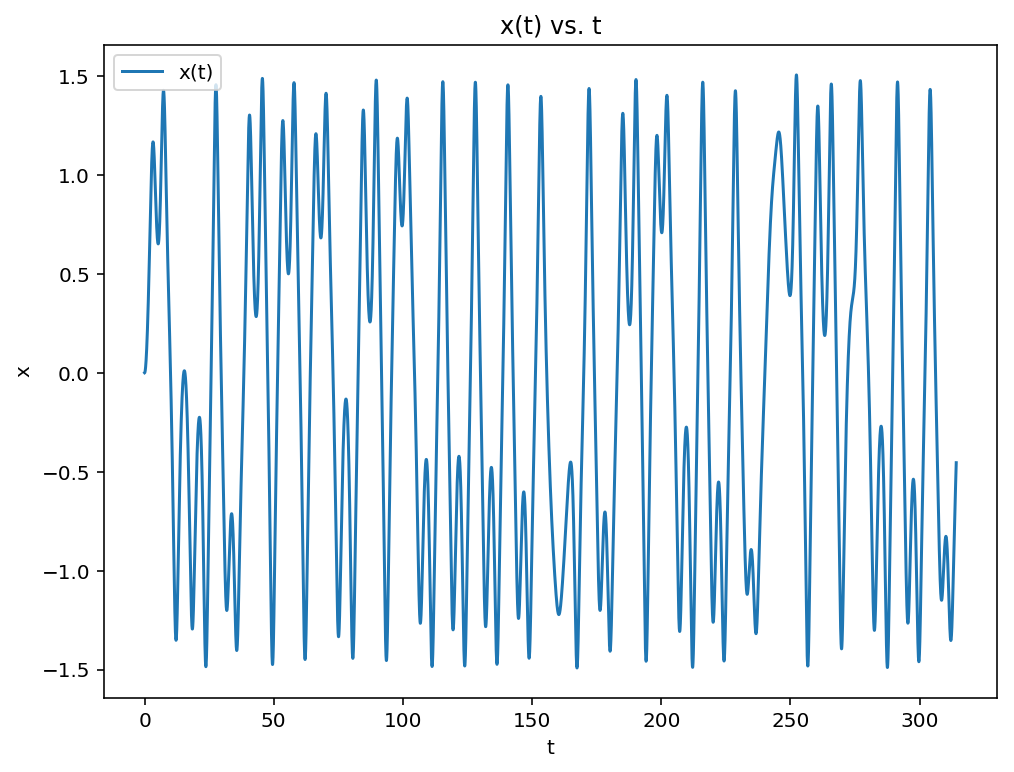
\includegraphics[scale=0.4]{x(t)6.png}
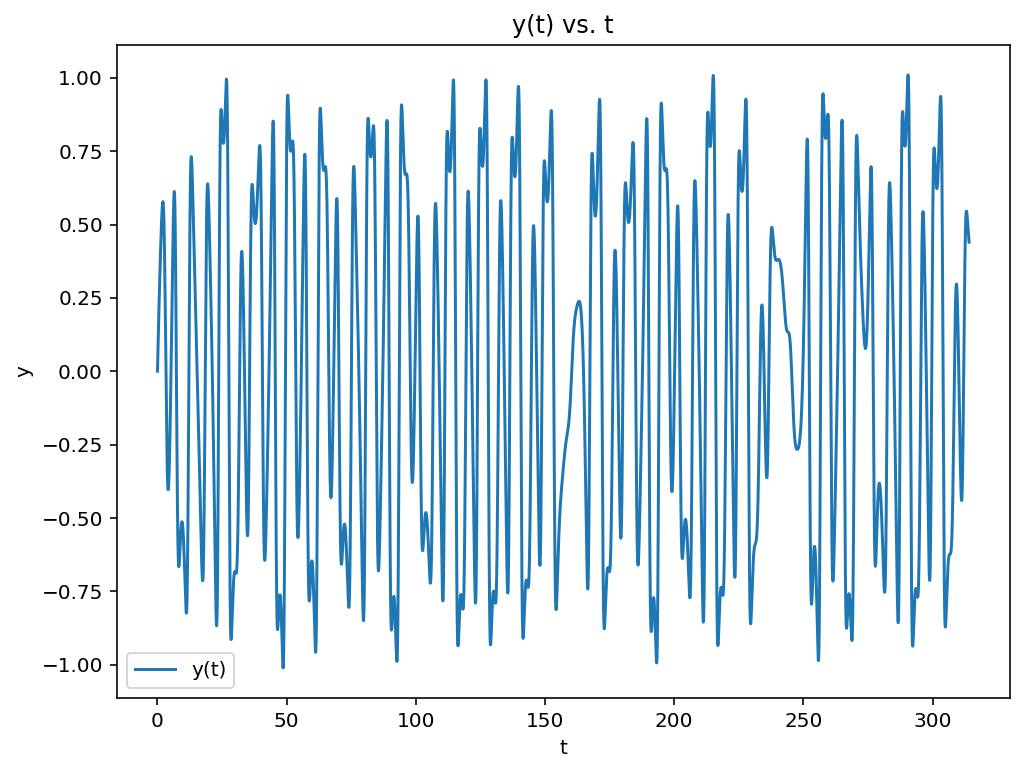
\includegraphics[scale=0.4]{y(t)6.png}
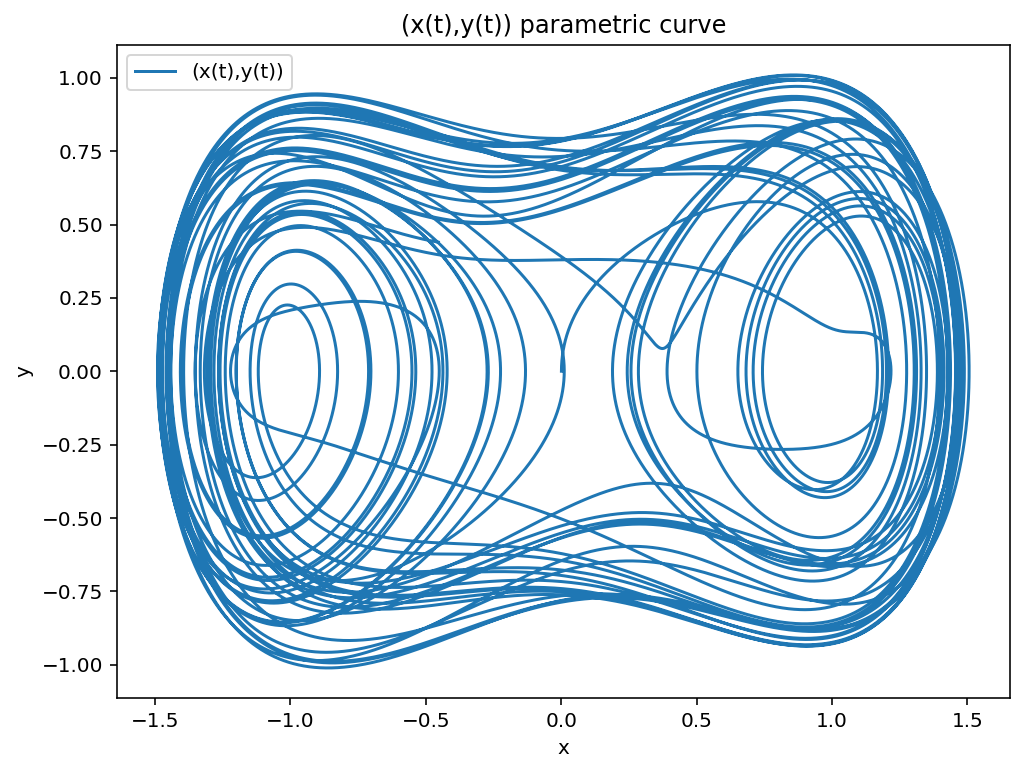
\includegraphics[scale=0.4]{parametriccurve6.png}
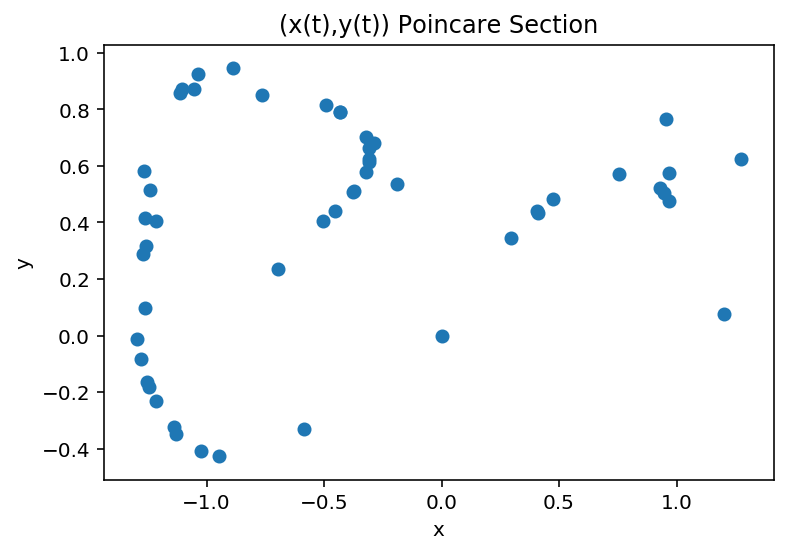
\includegraphics[scale=0.4]{poincare6.png}
\end{figure}

$F = 0.4$, $x(0) = 0.002$, and $y(0) = 0$

\begin{figure}[h!]
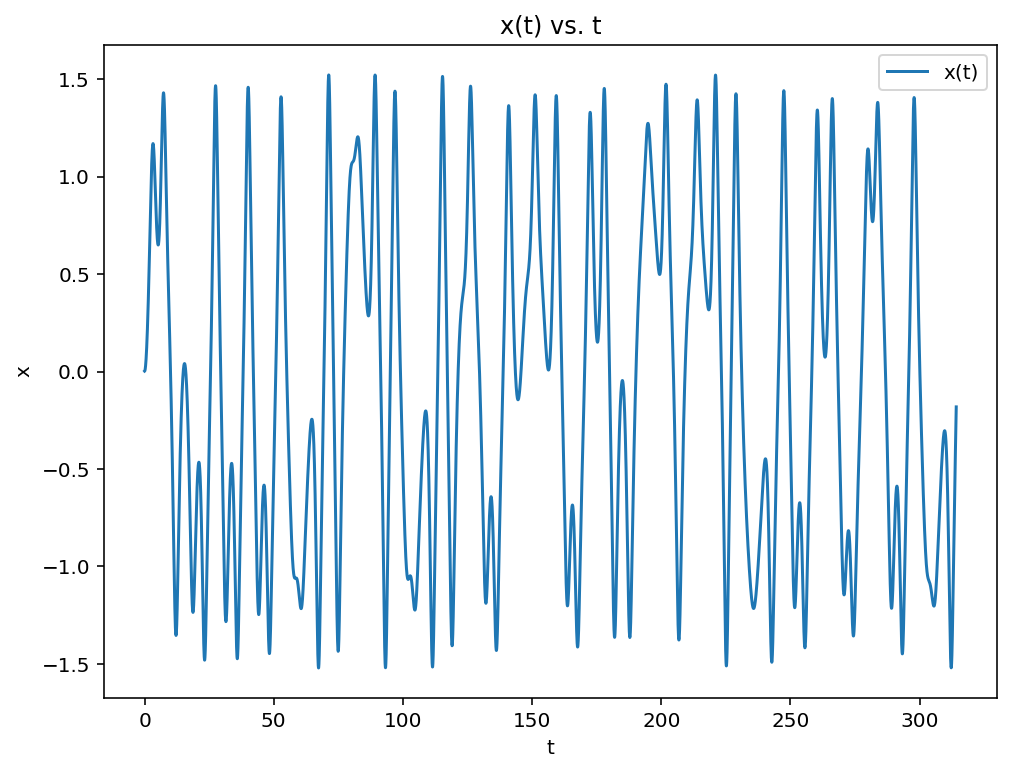
\includegraphics[scale=0.4]{x(t)7.png}
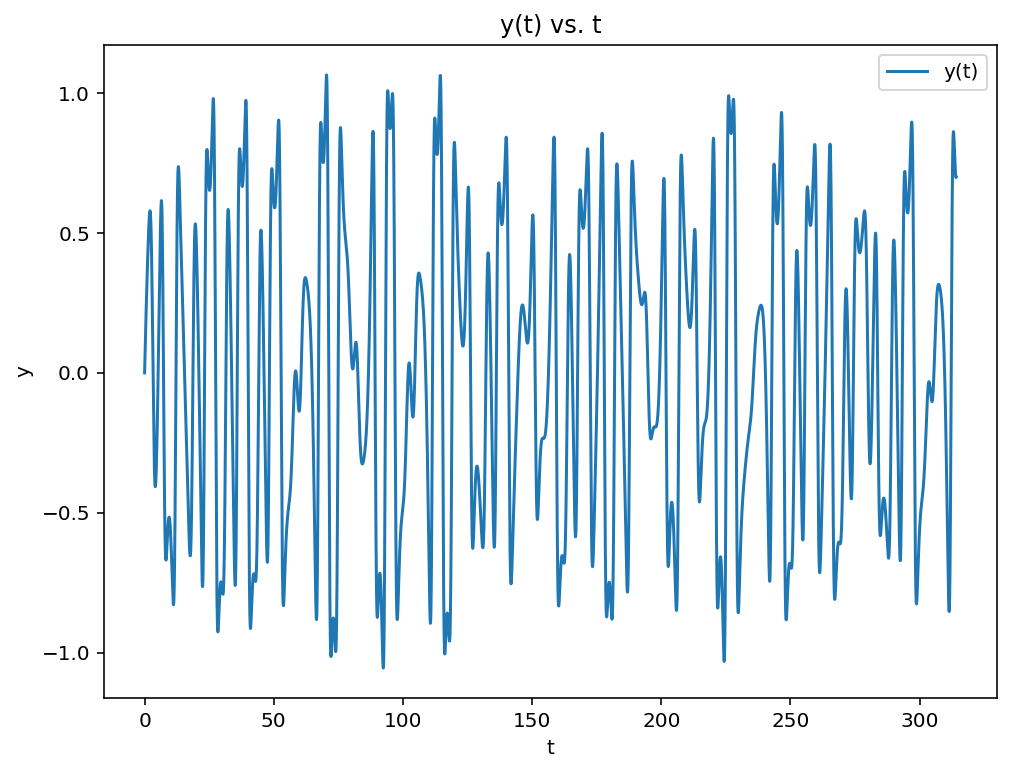
\includegraphics[scale=0.4]{y(t)7.png}
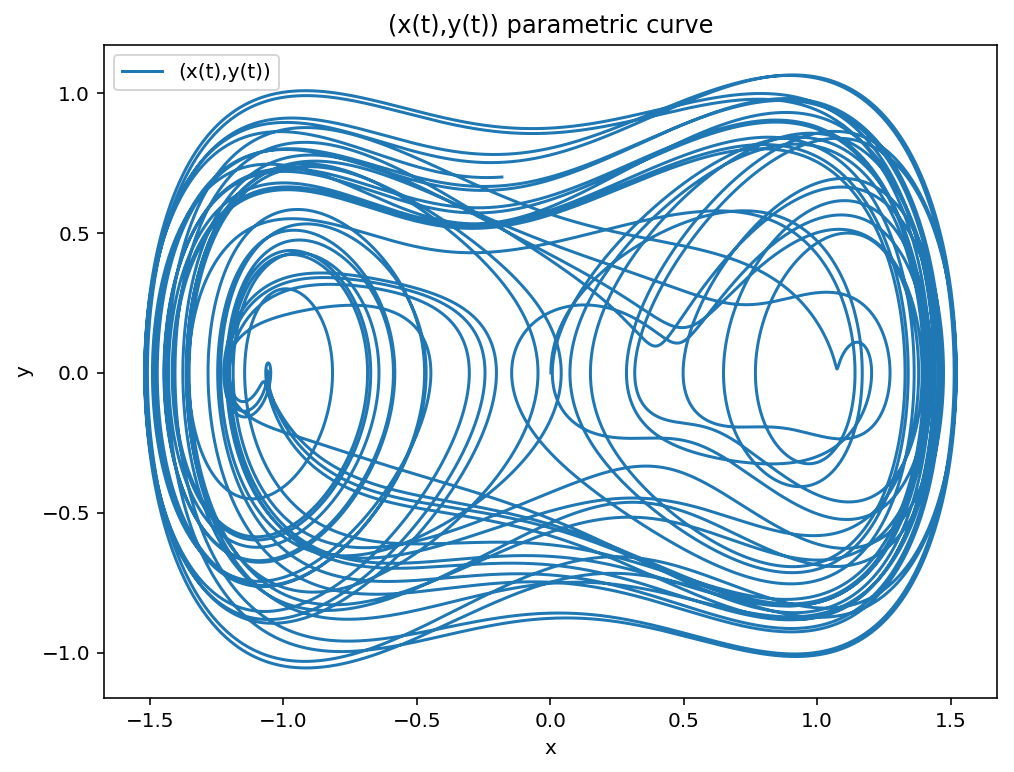
\includegraphics[scale=0.4]{parametriccurve7.png}
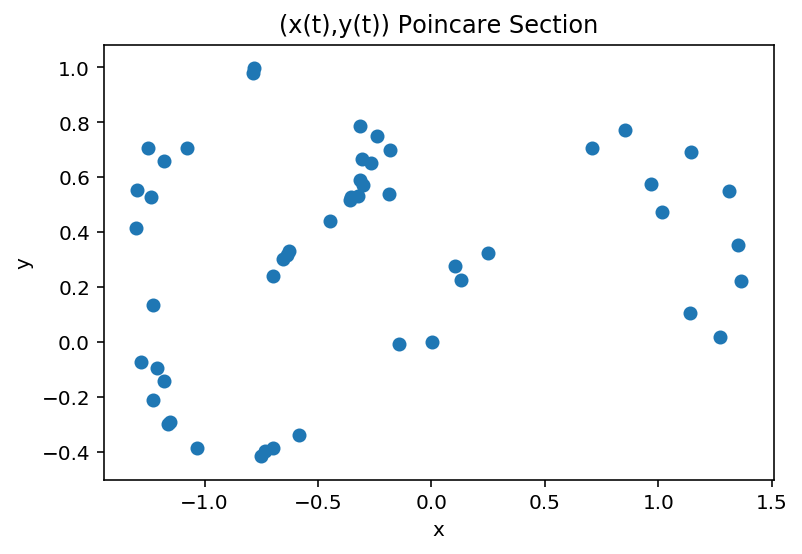
\includegraphics[scale=0.4]{poincare7.png}
\end{figure}

As we can see, the system is very sensitive to a tweak in initial conditions, a prime characteristic of chaos. Let's repeat the values $F = 0.4$, $x(0) = 0$, and $y(0) = 0$, with a time range $t\in[0,2\pi\, 1000]$ for a better examination of our Poincare section.

$t\in[0,2\pi\, 1000]$
$F = 0.4$, $x(0) = 0$, and $y(0) = 0$

\begin{figure}[h!]
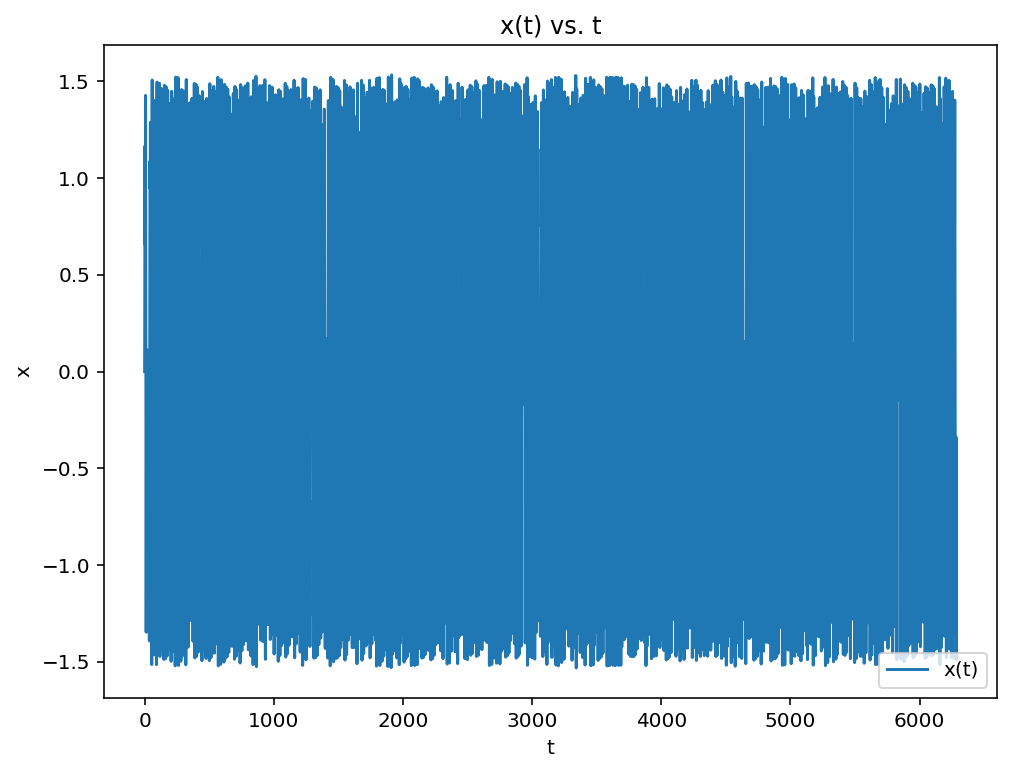
\includegraphics[scale=0.4]{x(t)8.png}
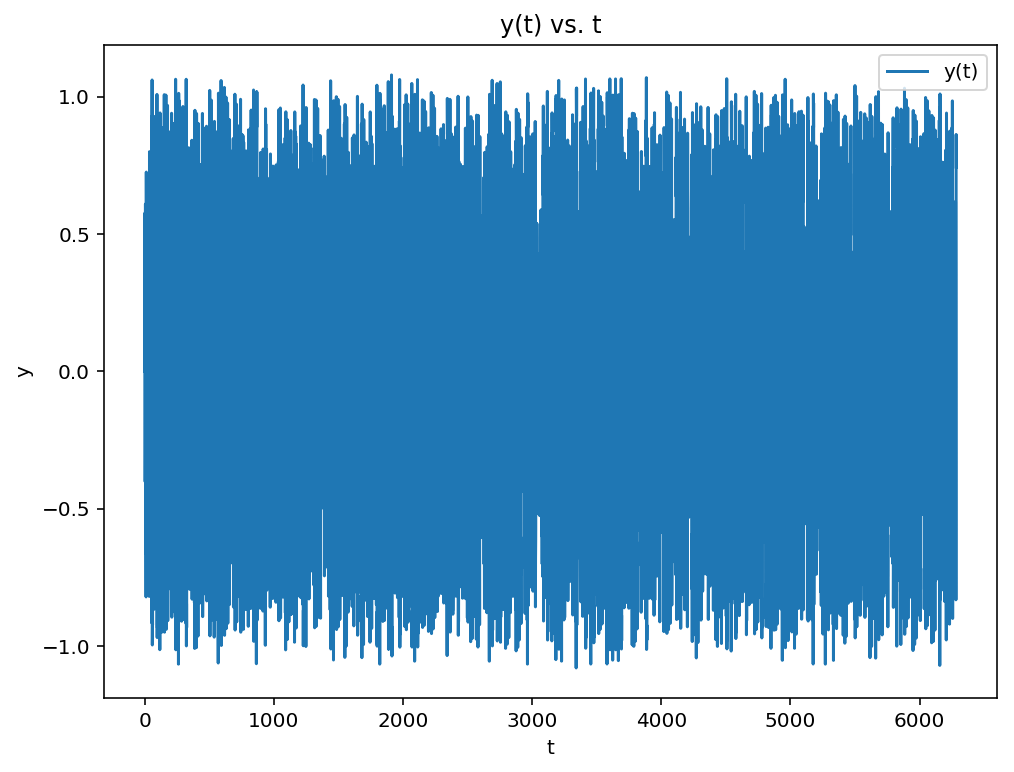
\includegraphics[scale=0.4]{y(t)8.png}
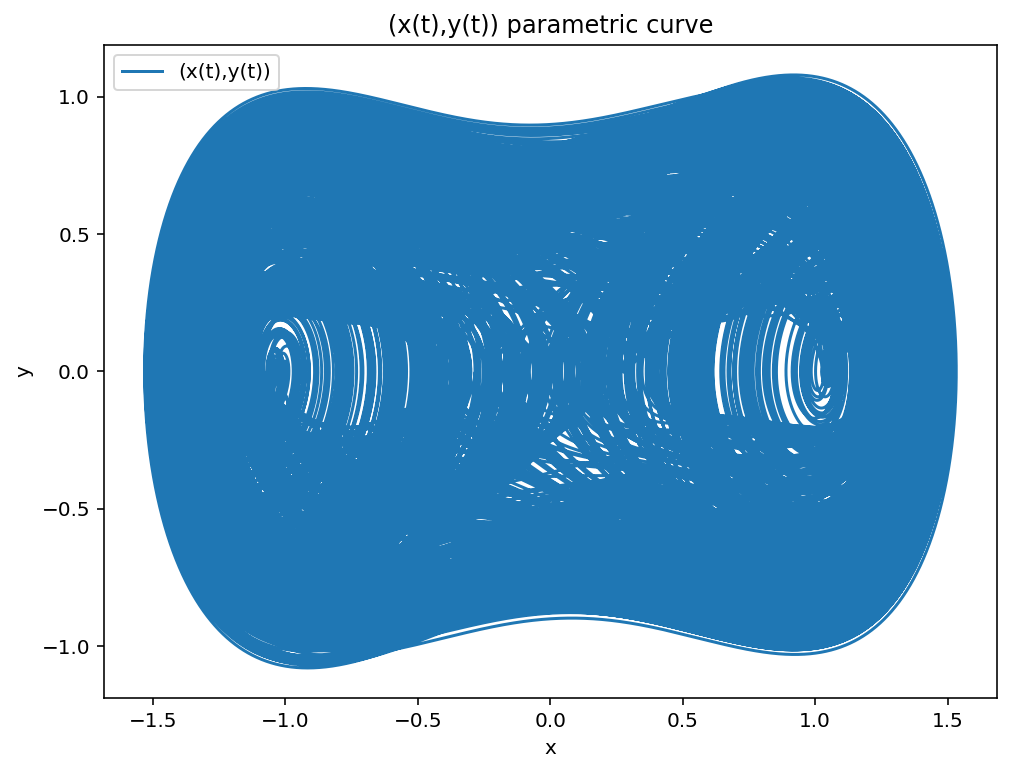
\includegraphics[scale=0.4]{parametriccurve8.png}
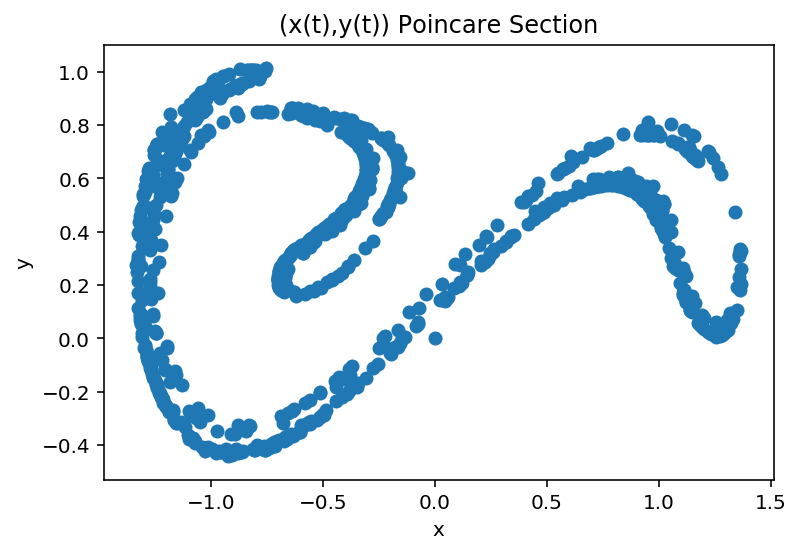
\includegraphics[scale=0.4]{poincare8.png}
\end{figure}

Now the Poincare section seems to be a great indication of a chaotic system.

\section{Conclusion}
As we can see, changing our driving force $F$ lead to a more chaotic system.
\end{document}
